% !TEX TS-program = Xelatex
% !TEX encoding = UTF-8 Unicode

\documentclass[UTF8]{ctexart}
\usepackage{amsmath}
\usepackage{dsfont}
\usepackage[table]{xcolor}
\usepackage[bottom]{footmisc}
\usepackage{graphicx}
\usepackage{figsize}
\usepackage{standalone}
\usepackage[separate-uncertainty = true,tight-spacing=true,round-minimum=0.00000000001]{siunitx}
\usepackage{tabu}
\usepackage{wasysym}
\usepackage{geometry}
\geometry{left=0.7in,right=0.7in,bottom=0.7in,top=0.7in}

\title{计算物理学作业2}
\author{朱寅杰 1600017721}
\date{2017年11月12日}

\begin{document}

\maketitle

\section{Runge效应}
我们使用各种方法来内插著名的Runge函数$R(x)=(1+25x^2)^{-1}$,并比较不同方法的误差大小。
\paragraph{多项式内插}
从-1到1每隔0.1取一个节点,作多项式插值。多项式使用Neville算法计算。程序文件为Neville.py。程序的前半部分产生了插值多项式,并计算了插值式从-1到1每隔0.05各处的值,并与实际的函数值一并列表于附表tabu1.1.pdf中。程序的后半部分使用Matplotlib包\footnote{Matplotlib: A 2D Graphics Environment” by J. D. Hunter In Computing in Science \& Engineering, Vol.9, No.3.(2007), pp.90-95.}作出了插值多项式在[-1,1]上的图像。可以看到这个多项式在$\lvert x \rvert >0.5$的时候就开始剧烈地偏离函数的实际值。

\paragraph{使用Chebyshev多项式内插}
仍然是使用多项式进行内插,只不过这次所用内插函数不再使用$\{1,x,x^2,...\}$这组基底,而是换用Chebyshev多项式$T_n=\cos(n\arccos(x)$为基底,节点也换成$\cos(\pi(k+1/2)/20),k=0,1,...19$。利用Chebyshev多项式的正交归一关系计算出具体的系数,并使用秦九韶算法(书上叫Clenshaw迭代)计算出插值多项式的值。程序文档为Chebeshev.py,计算了各节点及相邻节点中点的插值多项式的值,与实际函数值一并列于附表tabu1.2.pdf中。同样也作出了插值多项式在[-1,1]上的图像。可以看出这次的插值多项式就和实际函数吻合得很好。

\paragraph{使用三次样条函数内插}
这次改用三次样条函数进行内插。节点仍然是从-1到1每隔0.1,设出各节点处样条函数的矩(二阶导数值),用节点处连续可导排出一个三对角矩阵,用Thomas法求解之,然后积分算出样条函数。程序文件为spline.py。对于Runge函数我们将样条函数的边界条件取为在区间左右端点处的一阶导数值与原函数的相等,对应着代码中Spline函数中method="align"一段。计算了各节点及相邻节点中点的样条函数的值,与实际函数值一并列于附表tabu1.3.pdf中。同样也作出了样条函数在[-1,1]上的图像。可以看出样条函数与实际函数吻合得还要好。
\section{样条函数画心脏线}
使用三次样条函数内插心脏线的参数方程
$\begin{cases}
x(t)=(1-\cos t)\cos t\\
y(t)=(1-\cos t)\sin t
\end{cases}$。节点取为$t=n\pi/4,n=0,1,2,...,8$。由于此时样条函数应当满足周期边界条件,因此各节点的矩(样条函数二阶导)满足的方程组也是一个“周期性”的三对角方程,具有类似
\begin{equation*}
Ax=d,A=
\begin{bmatrix}
a&b&&&...&&&c\\
c&a&b&&...&&&\\
\vdots&\vdots&\vdots&\vdots&&\vdots&\vdots&\vdots\\
&&&&...&c&a&b\\
b&&&&...&&c&a
\end{bmatrix}
\end{equation*}
的形式。这样的系数矩阵虽然比一般的三对角矩阵对称性更高(划掉),但却不能直接使用Thomas方法进行$LU$分解。为此我们使用一一个网上找到的小技巧\footnote{https://www.cfd-online.com/Wiki/Tridiagonal\_matrix\_algorithm\_-\_TDMA\_(Thomas\_algorithm)}。
我们取$A'=A-uv^T$,其中$u^T=[-a,0,...,0,c]$,$v^T=[1,0,...,0,-b/a]$,分别求解$A'y=d$与$A'q=u$,则可以通过Sherman-Morrison公式计算出$x=y-\frac{v^Ty}{1+v^Tq}q$。

程序文件为spline.py。样条函数的计算对应其中Spline函数的method="periodical"一段,用到了上述的计算技巧。按要求程序计算了在各节点与节点之间处的点的两个函数值(见附表tabu2.pdf),并作出了用样条函数近似画出的心脏线$(S_{\Delta}(X,t),S_{\Delta}(Y,t))$,见下图。
\begin{figure}[h]
  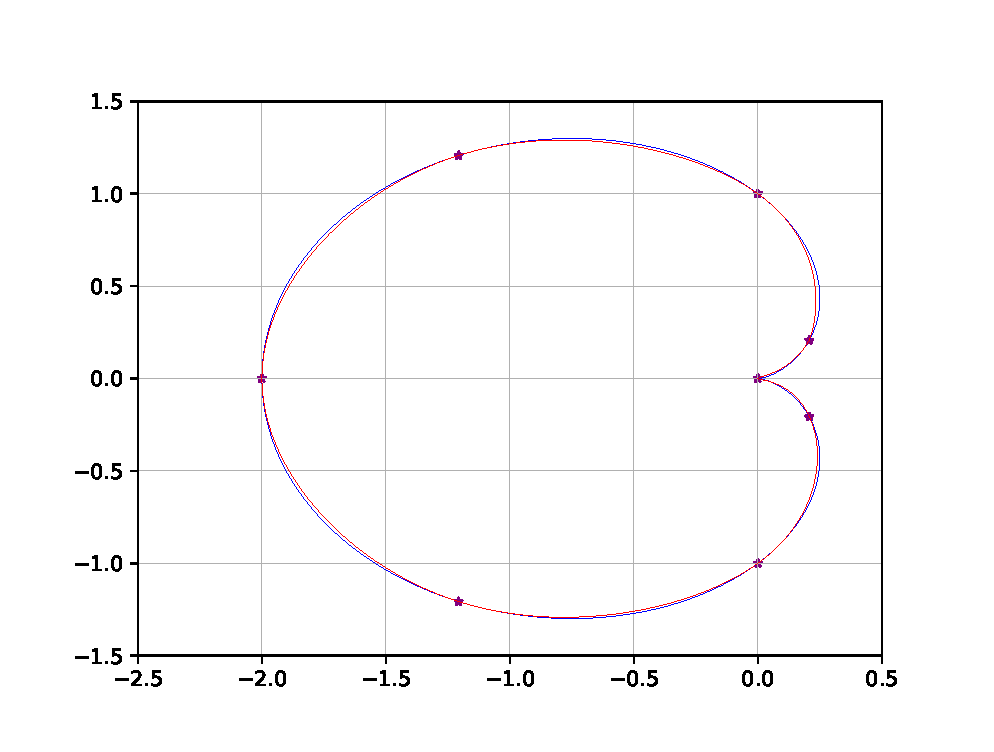
\includegraphics[width=\linewidth,keepaspectratio=true]{cardioid.eps}
  \caption{用样条函数内插绘制的心脏线图。图中蓝线为心脏线的准确形状,红线为用样条函数内插的结果。几个内插节点在图中使用星形标注。}
\end{figure}

样条函数能够很好地模仿函数的一阶与二阶导数行为(当然它不能很好地模仿更高阶的导数,但是由于一阶导数和二阶导数的行为对于作图来说是至关重要的,更高阶的导数对于图像的影响并不明显,所以对于作图而言这样的近似实际无伤大雅),并且又能保证在各个节点处的一阶导数与二阶导数均连续,因此画出的图像往往十分平滑而好看。
\section{含有Zeta函数方程的求解}
现在需要计算函数
\[
\mathcal{Z}_{00}(1;q^2)=\sum\limits_{\mathbf{n}}\frac{\exp{q^2-n^2}}{\sqrt{4\pi}(n^2-q^2)}-\pi+\frac{\pi}{2}\int_{0}^{1}t^{-3/2}\mathrm{d}t(\exp{tq^2}-1)+\pi\int_{0}^{1}t^{-3/2}\mathrm{d}t\times\frac{1}{\sqrt{4\pi}}\sum\limits_{\mathbf{n}\neq 0}\exp{-\frac{\pi^2n^2}{t}}\exp{tq^2}
\]
其中$\mathbf{n}\in\mathds{Z}^3$为三维整数。这个函数总共有四项,第二项是常数,第三项可展开为泰勒级数。
\[
\frac{\pi}{2}\int_{0}^{1}t^{-3/2}\mathrm{d}t(\exp{tq^2}-1)=\sum\limits_{n=0}^{\infty}\frac{q^{2n}}{(n-1/2)\times n!}
\]
对于第一项和第四项,在数值计算时涉及到一个对三维整数的求和,我们只能取有限的$\mathbf{n}\in\{-N,-N+1,...,N\}^3$。为了确定应当取多大的$N$,我们计算了取不同$N$不同$q^2$时函数的计算值,列于附表tabu3.1.pdf中。这部分工作对应Zeta.py的第一部分。从表中可以看出,至多取到$N=3$时可以保证有六位有效数字,至多取到$N=5$时可以保证有12位有效数字。具体对于某一个$q^2$应当取多少可以从附表中看出。

从表中我们可以看出,所求的函数在$q^2=0,1,2,3$处均有奇点,在(0,1)、(1,2)、(2,3)上分别由负无穷递增至正无穷。在$q^2=0$处,函数的行为接近于$\mathcal{Z}_{00}(1;q^2)\propto q^{-2}$。

由于函数的单调性很好,我们采用对分法求方程$\mathcal{Z}_{00}(1;q^2)=1+q^2/4$在$q^2\in(0,1)$上的解。这部分工作对应的是Zeta.py的第二部分。计算所得的结果为$q^2=\num{0.7945156579150956}$。注意:由于计算时所采用的精度比较高(取了$N=6$,第四项积分切成了1000块使用Cotes公式计算),因此耗时会比较长。

\begin{figure}
\centering
\SetFigLayout{3}{1}
\subfigure[使用多项式内插的结果。]{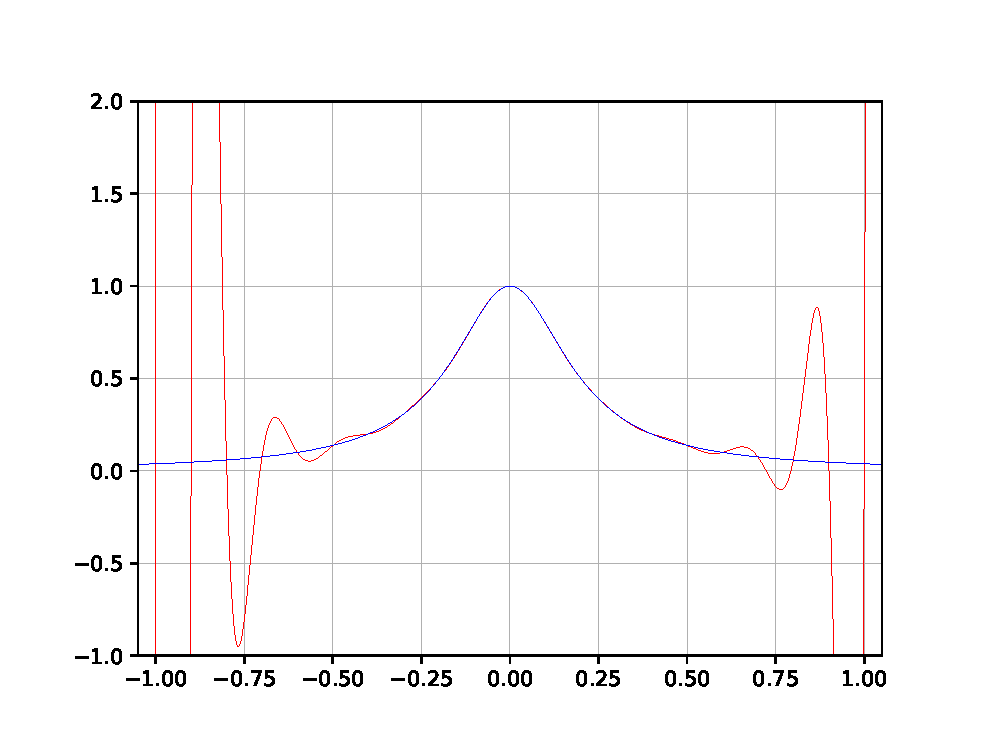
\includegraphics{Neville.eps}} \\
\subfigure[使用切比雪夫多项式内插的结果。]{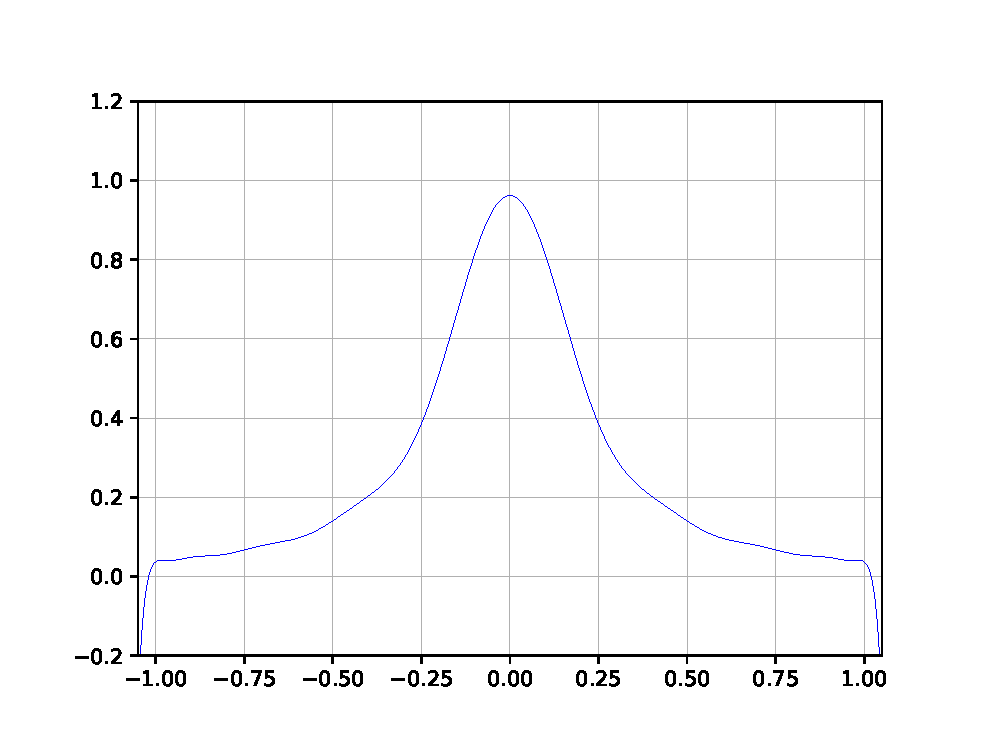
\includegraphics{Chebeshev.eps}} \\
\subfigure[使用样条函数内插的结果。]{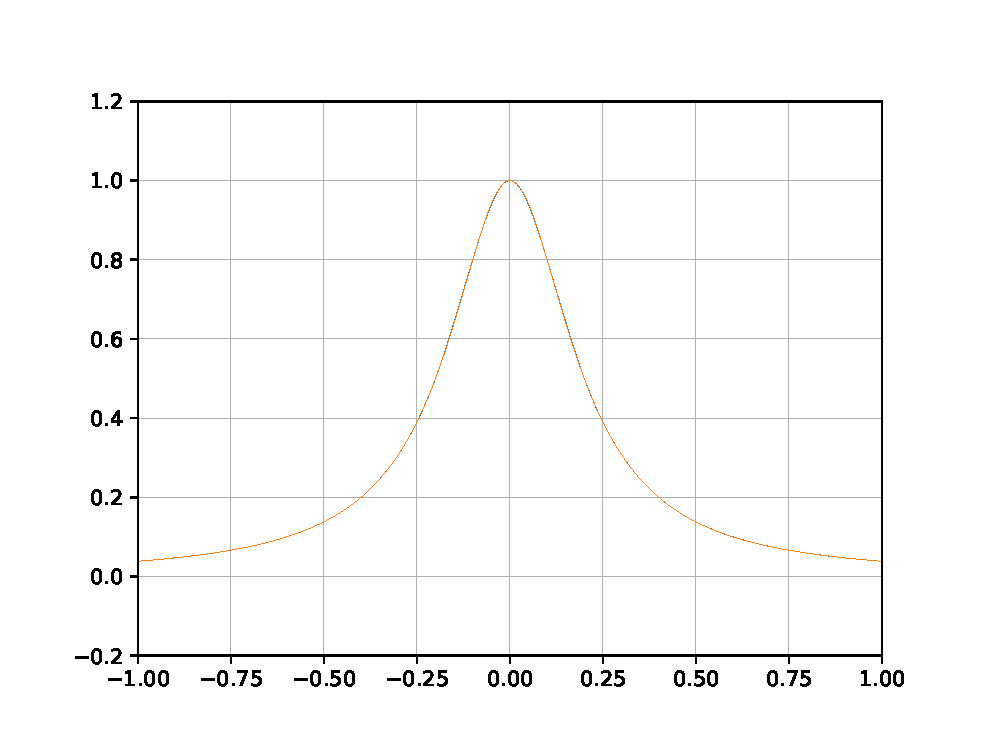
\includegraphics{spline.eps}} \\
\caption{使用不同方法对Runge函数内插的结果。蓝色为实际值,红色为内插值。}\label{fig:1}
\end{figure}

\end{document}


